\chapter{现场情况简介}

循环流化床锅炉是一种由鼓泡流化床发展起来的清洁燃烧技术,能够大大减少燃煤电站~\ce{NOx}和~\ce{SO2} 的生成量和排放量。与煤粉炉相比,循环流化床锅炉的主要不同点在燃烧系统。现场采用的锅炉为东方锅炉厂的100$\,$\si{\mega\watt}~ 级循环流化床锅炉,其型号为~DG410/9.81-\Rnum{2} 1,锅炉的主要设计性能指标如表~\ref{tab:cfbb}~所示。
\begingroup
\renewcommand*{\arraystretch}{1.67}
\begin{table}[!h]
\small
\centering
\caption[循环流化床锅炉主要设计指标]{循环流化床锅炉主要设计指标} \label{tab:cfbb}
\begin{tabular}{c|c}
\hline\hline
铭牌出力    &   410$\,$\si[per-mode=symbol]{\tonne\per\hour} \\
%\hline 
最大连续蒸发量 &   440$\,$\si[per-mode=symbol]{\tonne\per\hour} \\
%\hline 
额定蒸汽压力  &   9.81$\,$\si{\mega\pascal} \\
%\hline 
燃煤量 &   52.9$\,$\si[per-mode=symbol]{\tonne\per\hour} \\
%\hline 
石灰石耗量   &   8.5$\,$\si[per-mode=symbol]{\tonne\per\hour} \\
%\hline 
脱硫效率    &   95$\,$\si{\percent} \\
%\hline 
过量空气系数  &   1.20 \\
%\hline 
锅炉保证热效率 &   91$\,$\si{\percent} \\
%\hline 
额定蒸汽温度  &   540$\,$\si{\degreeCelsius} \\
%\hline 
给水温度(B-MCR)  &   215$\,$\si{\degreeCelsius} \\
%\hline 
冷渣器出口渣温 &   $\leq$150$\,$\si{\degreeCelsius} \\
%\hline 
煤粉粒度    &   $\leq$8$\,$\si{\mm},  $d_{50} = $1.2$\,$\si{\mm} \\
%\hline 
石灰石粒度   &   $\leq$1.5$\,$\si{\mm},  $d_{50} = $0.45$\,$\si{\mm} \\
\hline\hline
\end{tabular}
\note{$d_{50}$为累计量为50$\,$\si{\percent}~时的煤粒直径}
\end{table}
\endgroup


\section{循环流化床锅炉简介}

\subsection{锅炉整体布置}

该锅炉为单汽包锅炉、采用自然水循环,整体左右对称,其结构示意图见图~\ref{fig:cfbb}。

炉膛内布置有受热面,用于吸收燃烧释放的热量。炉膛壁布置有石灰石和给煤口,炉膛底部是水冷风室,两侧分别布置滚筒冷渣器。锅炉的高温过热器和低温过热器布置在尾部竖井中,饱和蒸汽在其中变成过热蒸汽。锅炉还设有喷水减温器,用于控制过热蒸汽温度。省煤器和空气预热器也布置在竖井,进一步吸收高温烟气的热量,降低排烟温度。

\begin{figure}[!htb]
\centering
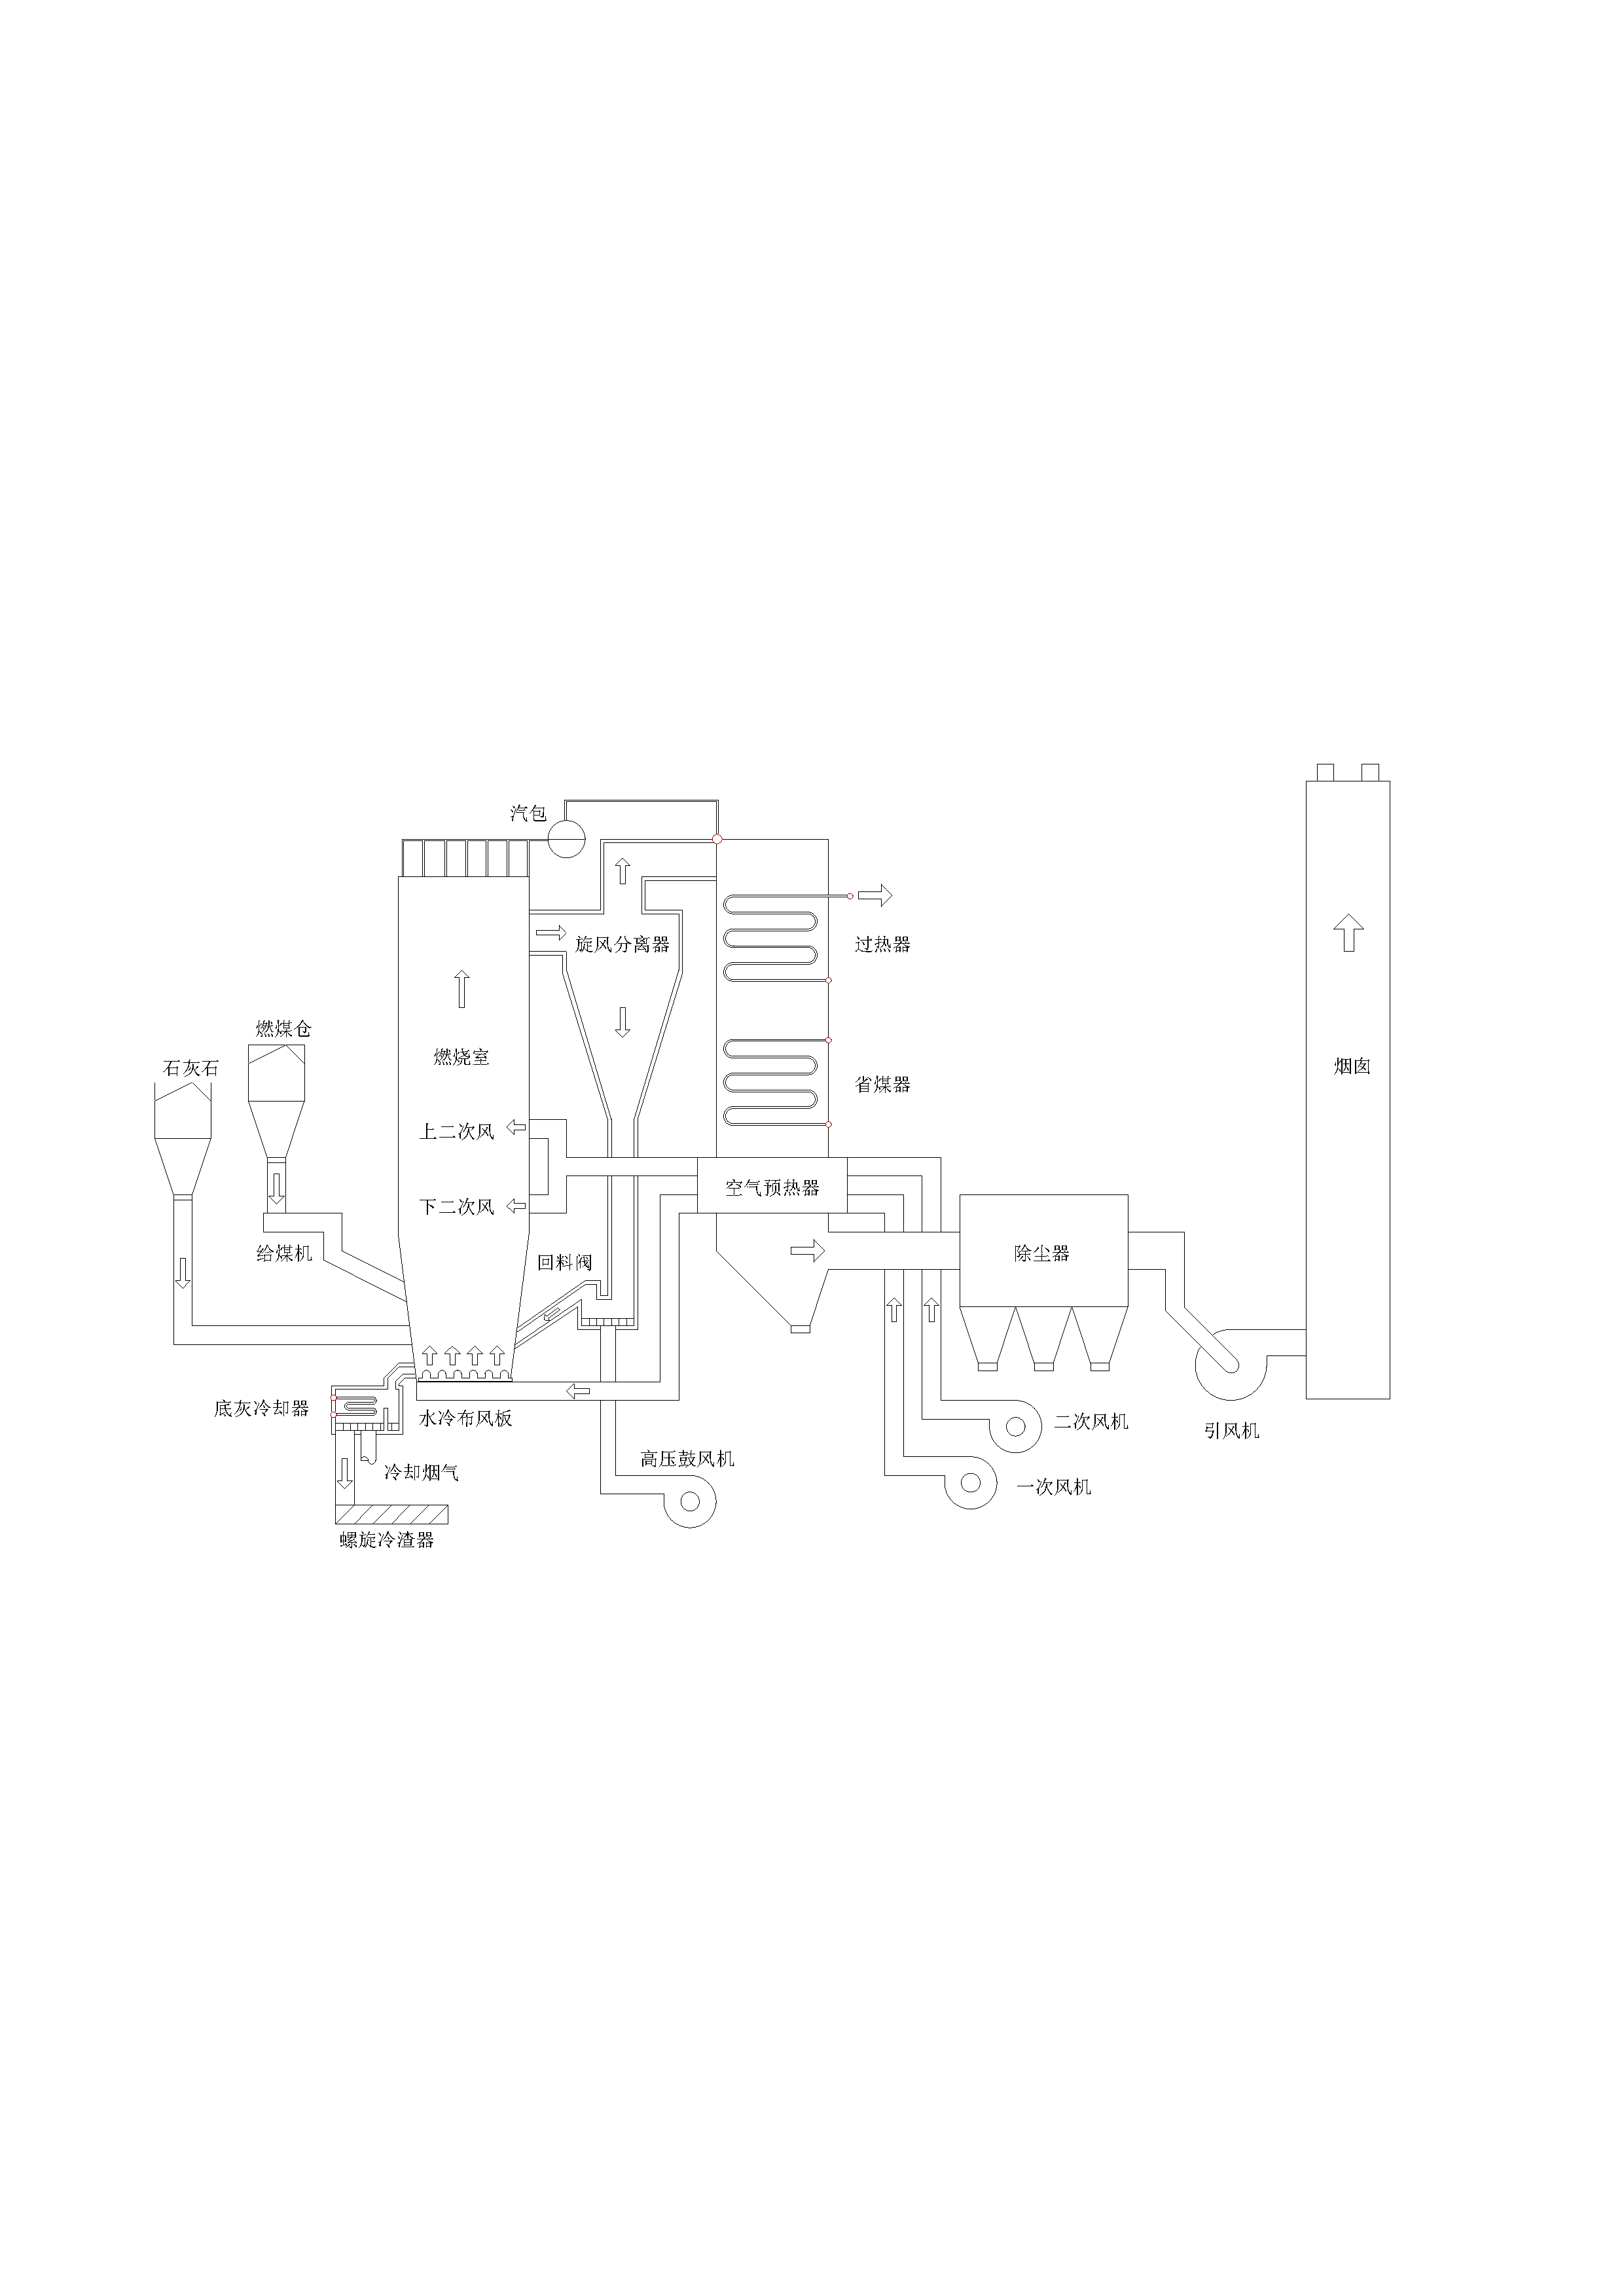
\includegraphics[width=14cm]{cfbb}
\caption{循环流化床锅炉结构示意图} \label{fig:cfbb}
\end{figure}

\subsection{燃烧系统}

锅炉的燃烧主要分布在两个区域:炉膛底部的密相区和炉膛上部的稀相区。破碎后的煤粒和脱硫所用的石灰石由给料口送入,一次风从水冷布风板进入,二次风分上下两层分布。锅炉的输煤线路有六条,均按25$\,$\si{\percent}~最大负荷容量设计。石灰石输送线路有三条。通过调整给料机的转速,可以控制锅炉的石灰石量和给煤量。

一次风除了用于维持床料颗粒的流化状态,也提供密相区燃烧所用的氧气。二次风主要作用是进一步补充煤粒燃烧所需的氧气。二次风的分层分布营造出炉内的密相区和稀相区底部的局部还原性气氛,从而减少~\ce{NOx}生成。在锅炉最大出力工况下,设计一次风占比约为总风量的55$\,$\si{\percent}。

煤粒进入炉膛后,在一次风的作用下迅速流化,并在密相区部分燃烧破碎释放热量。与此同时,石灰石在高温下分解生成~\ce{CaO}和~\ce{CO2}。煤中的硫燃烧产生~\ce{SO2},直接与~\ce{CaO}反应生成~\ce{CaSO4},实现了炉内脱硫。未燃尽的煤粒随一次风进入稀相区,与二次风混合后进一步燃烧,产生大量的高温烟气。高温烟气携带着煤粒和石灰石粒进入旋风分离器进行气-固分离。

固态床料被旋风分离器分离出来,通过J形回料阀返回炉膛实现燃料循环。燃烧产生的炉渣以及~\ce{CaSO4}经冷渣器排渣口排除锅炉,以维持固定的床层压力。另外,回料器还有床料补充口,在床料不足时可以由此处补充床料。


\subsection{汽水系统}

锅炉为自然循环锅炉,水循环借助自身重力,不需要额外的动力。水通过省煤器首次加热,接着进入锅炉汽包。汽包中的水沿下降管进入炉膛内的水冷壁,并在其中被加热成为汽水混合物,水的流动就是依靠其自身的密度差实现的。汽水混合物向上流动,重新返回汽包进行汽水分离。分离出的蒸汽经低温过热器和高温过热器加热,成为符合工艺要求的过热蒸汽,接着进入生产的下游环节。分离出的水重新进入水冷壁,再一次进行汽水循环。

系统采用喷水减温来调节主蒸汽温度、保护受热面的管道。过热器系统分两级减温,一级减温器作为粗调,控制高温过热器入口的蒸汽温度;二级减温器作为一级减温的补充,控制高温过热器出口的蒸汽温度。

\subsection{风烟系统}

从一次风机鼓出的空气经空气预热器加热送入炉膛底部,维持床料流化状态。从二次风机鼓出的空气也由空气预热器加热,进入炉膛参与燃烧,并调整炉内温度分布,防止局部温度过高。

烟气及其携带的固态床料离开炉膛后进入旋风分离器。烟气里的粗颗粒进入J阀,经J阀送回到炉膛。而飞灰仍夹带在烟气中,进入尾部竖井后向下流动。随后高温烟气依次将热量传递给高温过热器、低温过热器、省煤器后,通过空气预热器进入除尘器,除去烟气中的颗粒物。最后,由引风机将烟气抽进烟囱,排入大气。

\subsection{脱硝系统}

该锅炉采用SNCR(Selective Non-Catalytic Reduction,选择性非催化还原法脱硝)技术实现烟气的脱硝处理,进一步降低系统的排放量。浓氨水与稀释水混合后作为还原剂,喷向旋风分离器出口的烟道。在高温环境下,还原剂迅速分解变成~\ce{NH3},~\ce{NOx}与~\ce{NH3}反应生成~\ce{N2}和~\ce{H2O}。

\section{现场控制系统简介}
锅炉采用的DCS(Distributed Control System,集散控制系统)为横河电机(中国)有限公司的 CENTUM CS 3000 R3 综合生产控制系统。该系统与用于水/煤灰处理的 GE PLC(Programmable Logic Controller,可编程逻辑控制器)通过OPC接口接入工厂的 SIS(Supervisory Information System,监控信息系统)。

采用CENTUM CS 3000系统的典型网络拓扑结构如图~\ref{fig:cs3000}~所示。CS 3000提供了HIS(Human Interface Station,人机接口站)、现场控制站(Field Control Stations,FCS)、EWS(Engineering Workstation,工程师站)、V网和以太网等\cite{konishi2000system}。HIS主要提供操作监视功能,FCS主要负责装置的控制,ENG安装了CS 3000系统生成和维护管理功能,可以进行安装调试。V网是连接FCS、HIS、BCV(总线转化器)等的实时控制总线,具有高速响应性和高可靠性,系统可以通过BCV将其他域的CS 3000、CS 1000、$\mu$~XL系统等接入V网。以太网连接HIS、EWS以及上位信息系统\cite{emori1997communication}。

\begin{figure}[!htb]
\centering
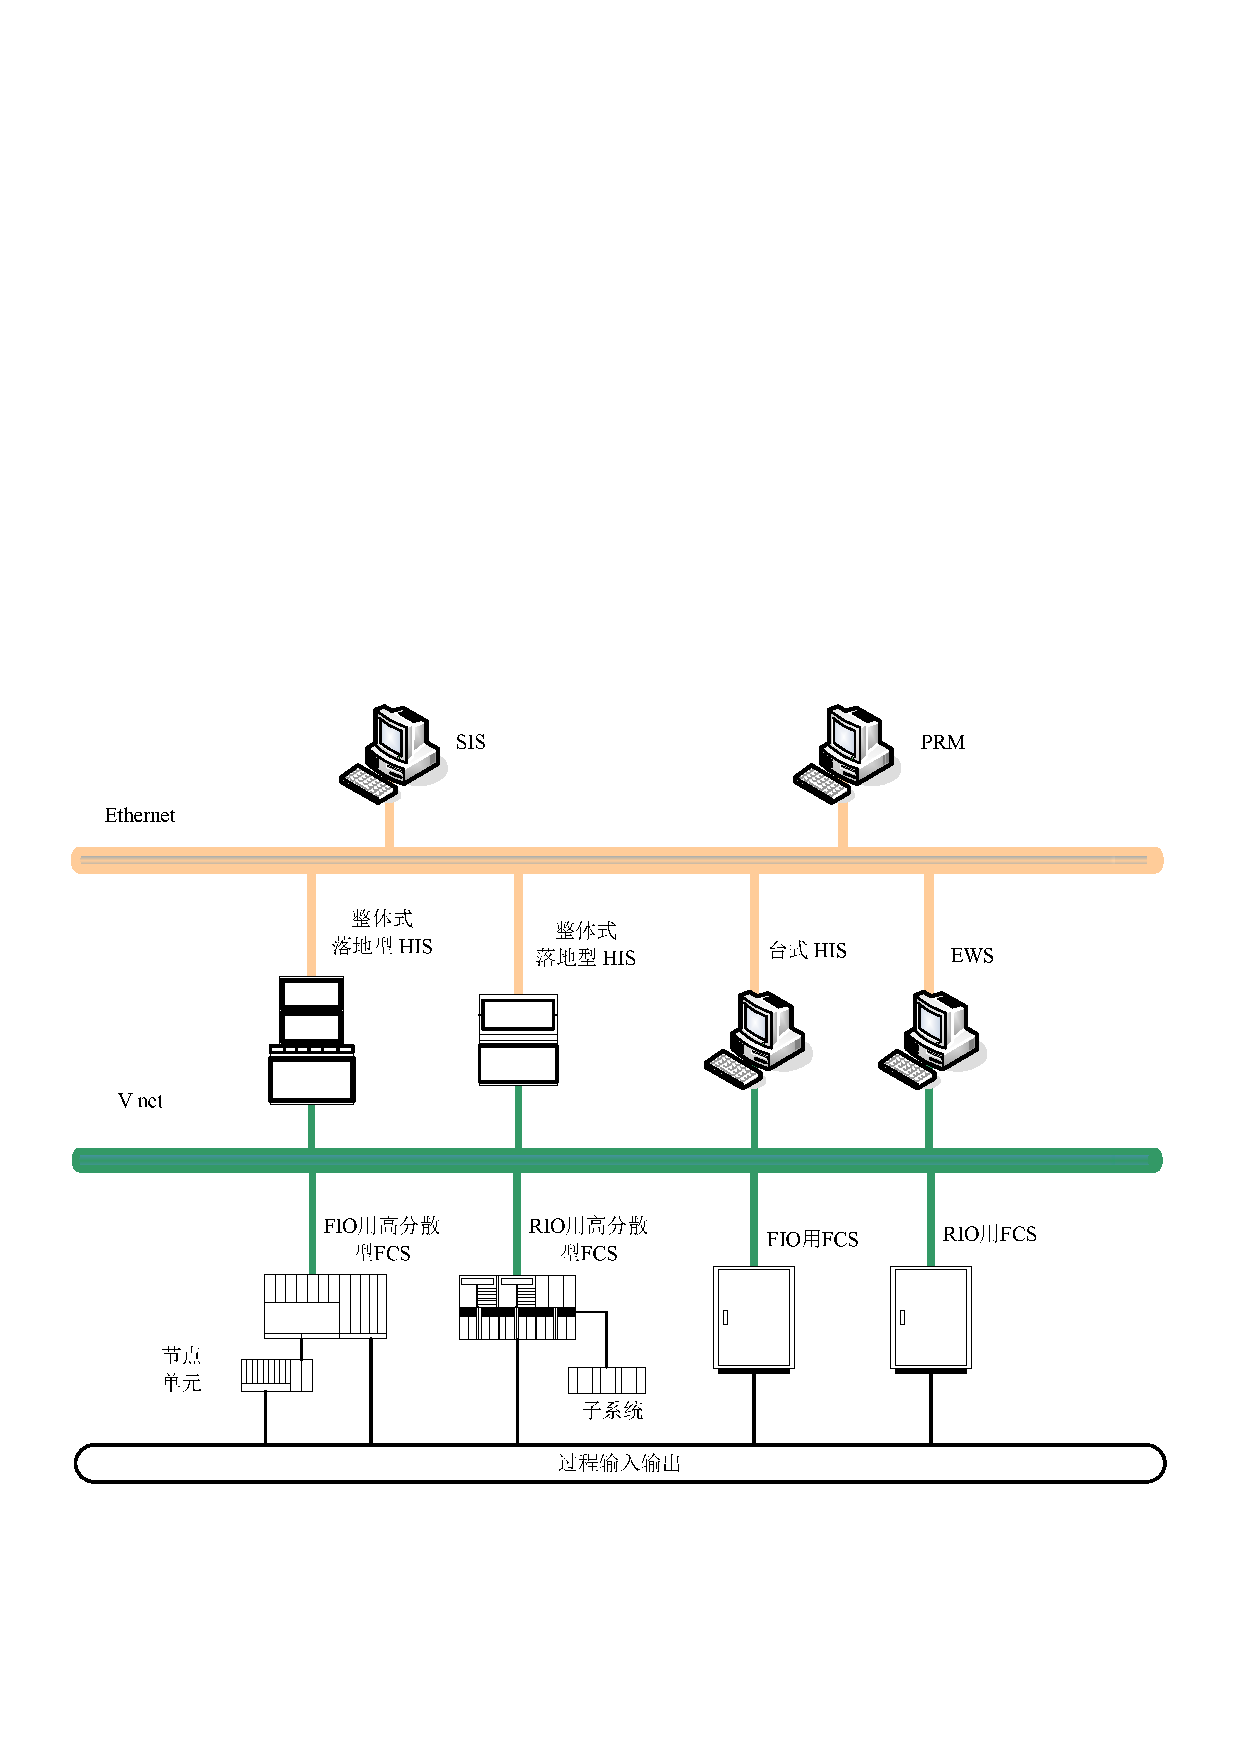
\includegraphics[width=13cm]{cs3000}
\caption{CS 3000架构} \label{fig:cs3000}
\end{figure}

HIS提供了丰富的过程监视/操作功能,除了系统信息和帮助外,还提供了过程报警、过程总貌、趋势图、流程图、顺序表、操作指导等窗口。此外,还提供了报告、画面拷贝等操作支持功能和报表、DDE(Dynamic Data Exchange,动态数据交换)、OPC等扩展功能。

FCS是实现控制功能的核心。它提供了多种执行控制运算的功能块,工程技术人员将连续控制块、顺控块和运算块结合起来就可以流程形式描述控制功能。连续控制块主要用于过程的监视和控制,其运算处理采用模拟量。顺控块提供顺序控制功能,使系统按照开发者预先规定的顺序逐步执行控制各阶段的操作。运算块主要作为辅助,提供对模拟信号或者数字信号的通用运算功能。常用的功能块如表~\ref{tab:fcs_blocks}~所示。

\begingroup
\renewcommand*{\arraystretch}{1.67}
\begin{small}
\begin{longtable}[!h]{l|p{11cm}}
% 首页表头
\caption[FCS常用控制块]{FCS常用控制块} \label{tab:fcs_blocks}\\

\toprule[0.5pt]
\hline
名称  & 说明 \\
\midrule
\endfirsthead
% 续页表头
\caption[FCS常用控制块(续)]{FCS常用功能块(续)} \\
\toprule[0.5pt]
\hline
名称  & 说明 \\
\midrule
\endhead
% 首页表尾
\hline
\multicolumn{2}{r}{\small 续下页}
\endfoot
% 续页表尾
\hline
\bottomrule[0.5pt]
\endlastfoot

PVI &   将输入信号作为测量值进行显示\\
PVI-DV  &   除PVI本身的功能外,还有“偏差报警”以及“设定值限幅”2种功能。\\
PID &   对偏差进行PID控制\\
MLD&输出设定的操作输出值(MV)\\
MLD-PVI&MLD-PVI块进行测量值(PV)和操作输出值(MV)的输出。一边监视测量值(PV),一边对操作端进行手动操作\\
MLD-SW&开关块,切换来自功能块等的信号和手操信号\\
VELLIM&将变化量限制在变化率限制值内后输出,避免信号发生突变\\
FOUT&用于串级控制,将串级信号分配给回路的下游的多个调节功能块中\\
LC64&用逻辑运算元件记录输入信号和输出信号的关系\\
RL&判定2个数据的大小或者逻辑关系\\
AVE&求输入数据的平均值\\
ADD&执行加法、减法运算\\
MUL&执行乘法运算\\
AND&在运算运算输入值(RV1,RV2)的逻辑与\\
NOT&执行否定运算\\
OR&运算输入值(RV1,RV2)的逻辑和\\
TON&在运算输入值(RV)由0变化为其它值时,只在1次扫描之间把运算输出值(CPV)设定为1\\
OND&在运算输入值(RV)由0变化为其它值后,经过预先设定的时间,将运算输出值(CPV)设为1\\
LAG&对输入信号执行1步滞后处理\\
CALCU&定义任意运算算法\\
DSET&用于信号的给定,通过操作监视功能输入任意数据\\
\end{longtable}
\end{small}
\endgroup
CS 3000提供的工程技术功能既可以与HIS共存,也可以独立安装在通用PC上, 其基本功能由系统视图和组态构成。系统视图按照树形结构显示项目工程文件。组态提供了对项目通用功能、操作监视、控制功能进行生成的能力。用户还可以利用调试功能对工程进行运行前的测试。CS3000还具备操作权限管理功能,对普通操作人员只提供HIS的操作监视功能,对工程师提供工程生成、修改和调试功能。

\section{燃烧系统控制现状}

现场DCS虽然有PID和手动控制两种控制手段,但实际上由于PID参数很久没有重新整定,燃烧系统大部分时段处于手动控制状态。

\subsection{主汽压力回路}

除了锅炉启动和停炉外,当锅炉正常运行时,维持合格的主蒸汽压力是燃烧系统的首要目标。对于该锅炉而言,最大出力状态下,正常的过热器出口蒸汽压力应维持在9.81$\,$\si{\mega\pascal}~$\pm$~0.1$\,$\si{\mega\pascal}。当锅炉负荷改变时,可以通过调节给煤量和风量来调节锅炉负荷。
 
目前主汽压力的控制与煤粉炉类似,都是通过调节给煤量来实现的,采用主汽压力—给煤量串级调节和PID控制器,如图~\ref{fig:gas_pre_pid}。在该串级控制回路中,主回路控制主汽压力,副回路控制给煤量,副回路并不比主回路响应迅速。此外,锅炉的主汽流量会对主汽压力产生较大影响,该控制策略并没有考虑主汽流量的影响。
\begin{figure}[!htb]
\centering
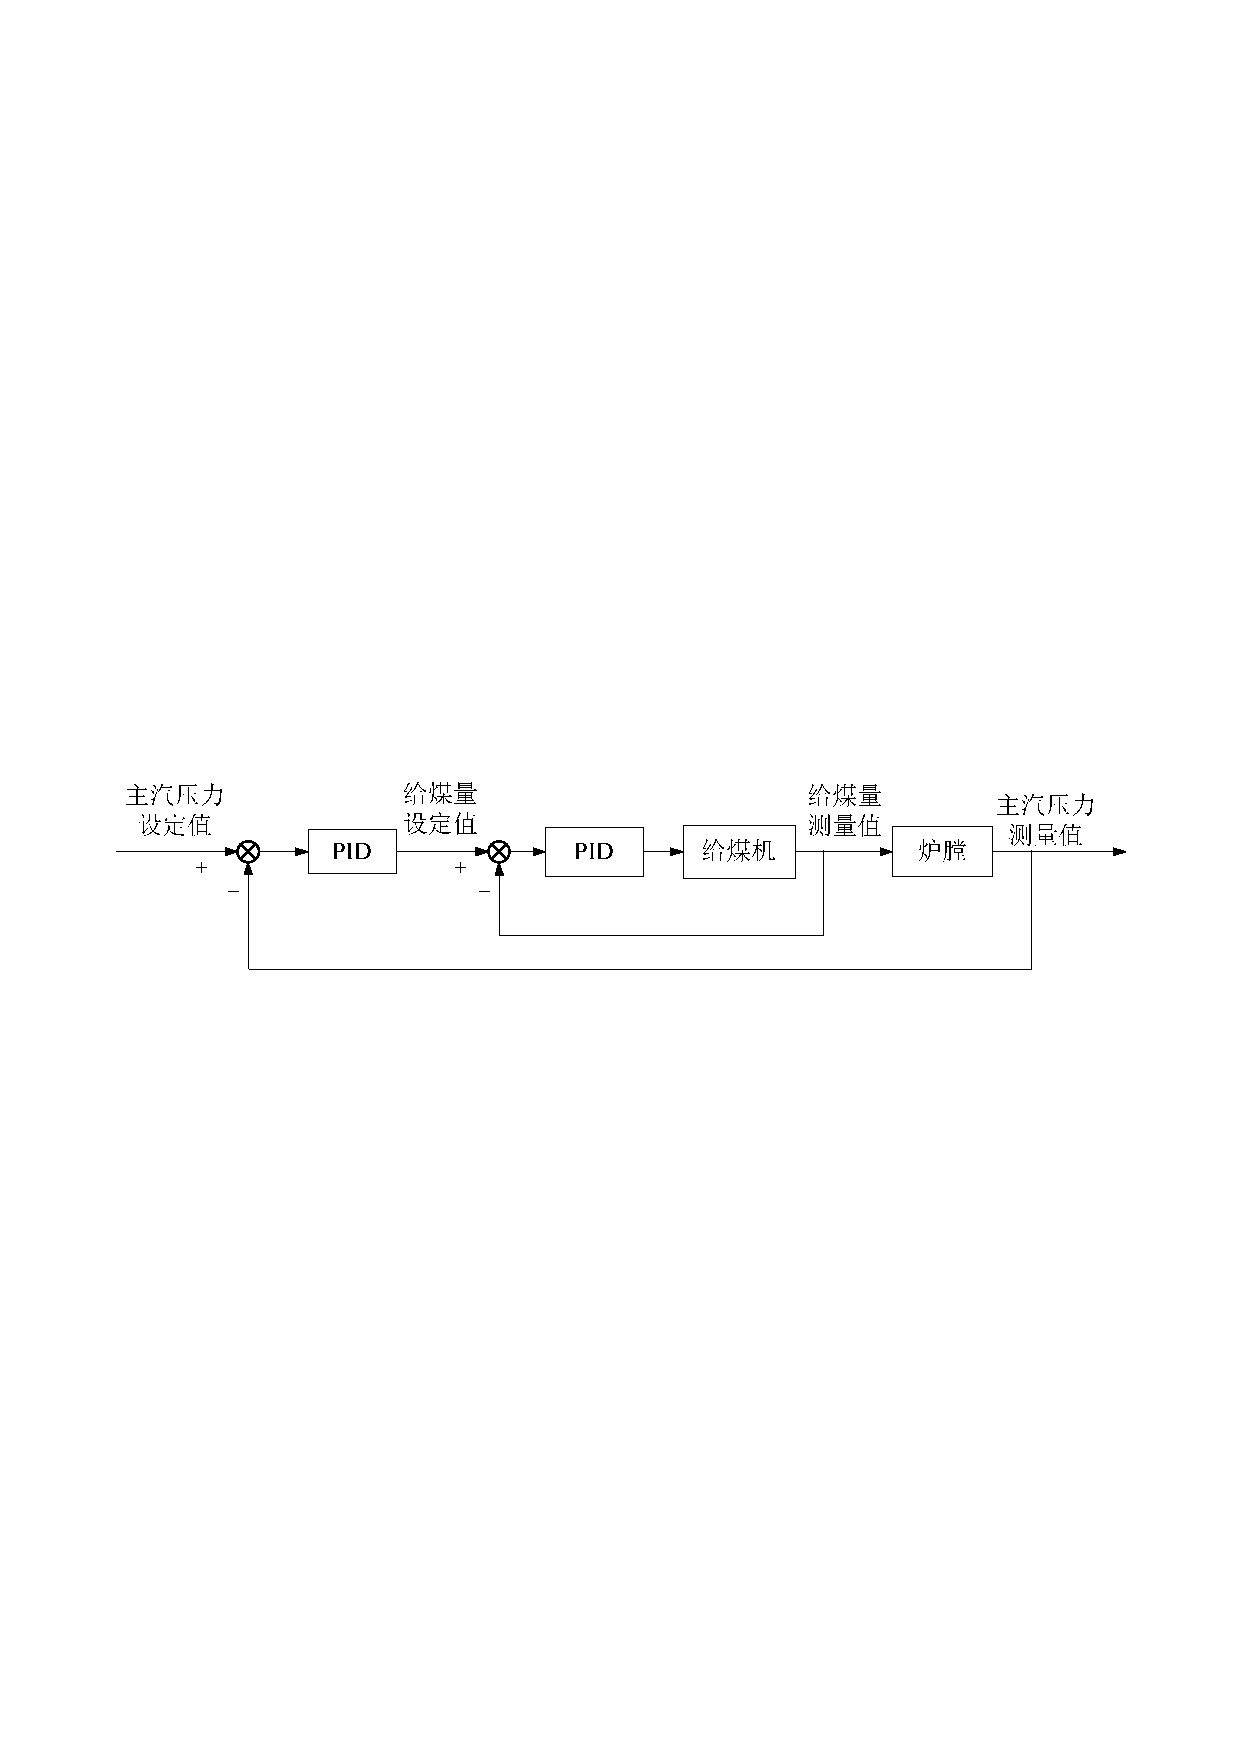
\includegraphics[width=13cm]{gas_pre_pid}
\caption{主汽压力回路PID控制策略} \label{fig:gas_pre_pid}
\end{figure}

图~\ref{fig:gas_pre_line_pid}~为某天主汽压力的变化曲线,可以看出主汽压力的波动非常大,在部分时刻甚至达到了0.3$\,$\si{\mega\pascal}。国标要求主汽压力的波动应在设定值上下0.1$\,$\si{\mega\pascal}~内,这样的运行状态会导致下游发电机运行不稳定,甚至导致生成事故。

\begin{figure}[!htb]
\centering
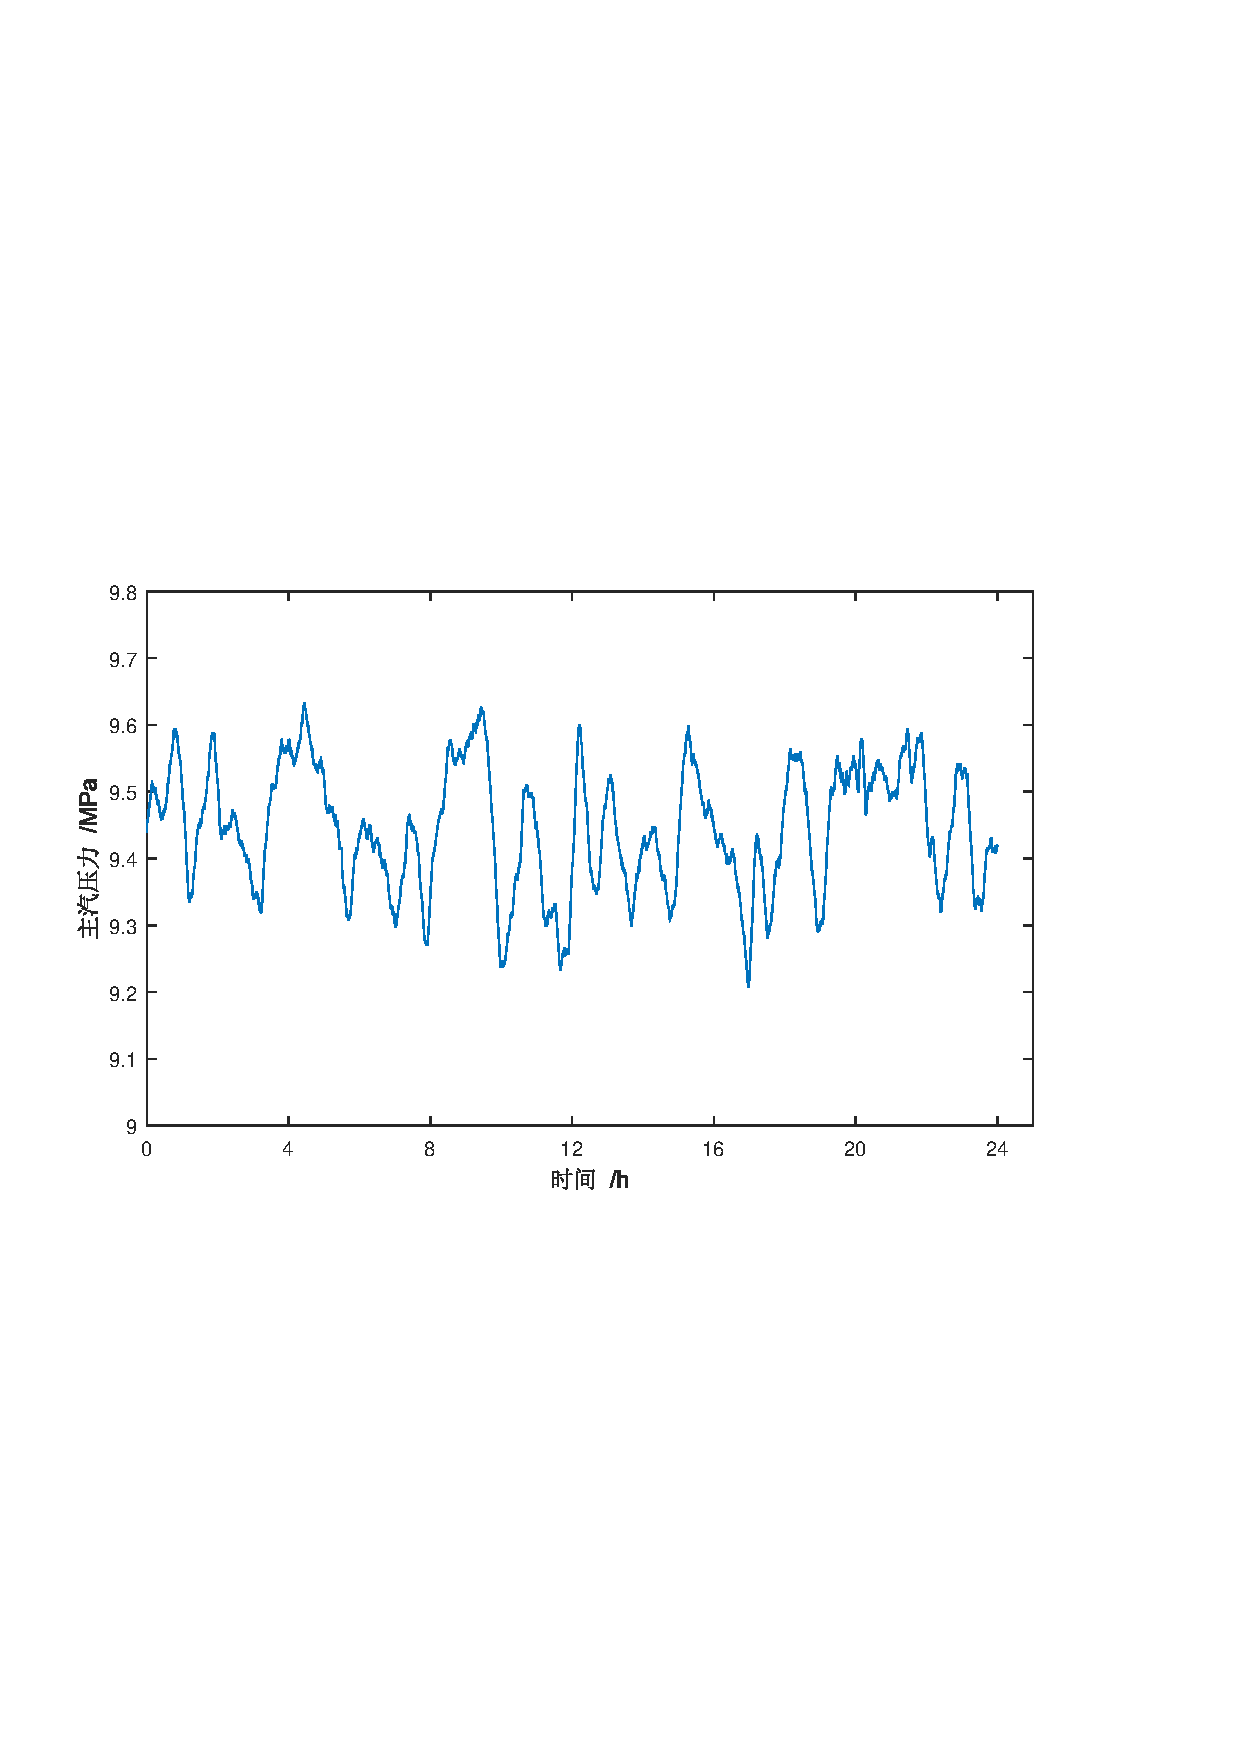
\includegraphics[width=12cm]{gas_pre_line_pid}
\caption{主汽压力回路控制效果} \label{fig:gas_pre_line_pid}
\end{figure}
 
\subsection{床温回路}
床温由24只床温热电偶测量,平均后作为床温信号。正常的床温范围在850$\,$\si{\degreeCelsius}~到935$\,$\si{\degreeCelsius}~之间,并且允许短时间内的大幅变化,以此来满足快速调节锅炉负荷的要求。但当达到所需负荷后,床温应当重新稳定在设定值附近。床温的设定值对循环流化床锅炉的运行有较大影响。床温过高,虽然会提高锅炉的热效率,但高床温会导致燃烧生成更多的~\ce{NOx},影响石灰石脱硫剂的脱硫效率,甚至导致炉膛内床料结焦,床层不能维持良好的流化状态,影响燃烧的持续稳定进行。床温过低会导致燃烧不完全,甚至锅炉灭火。
 
目前床温的控制是通过一次风来实现的,采用床温—一次风量的串级回路和PID控制器,如图~\ref{fig:bed_tem_pid}。单独使用一次风控制床温存在这样的问题:调节幅度小的话控制效果不明显;调节幅度大了则可能因为一次风和给煤量不匹配而影响到流化状态,也存在给煤没有快速跟导致上炉温上升后又快速回落的问题。
\begin{figure}[!htb]
\centering
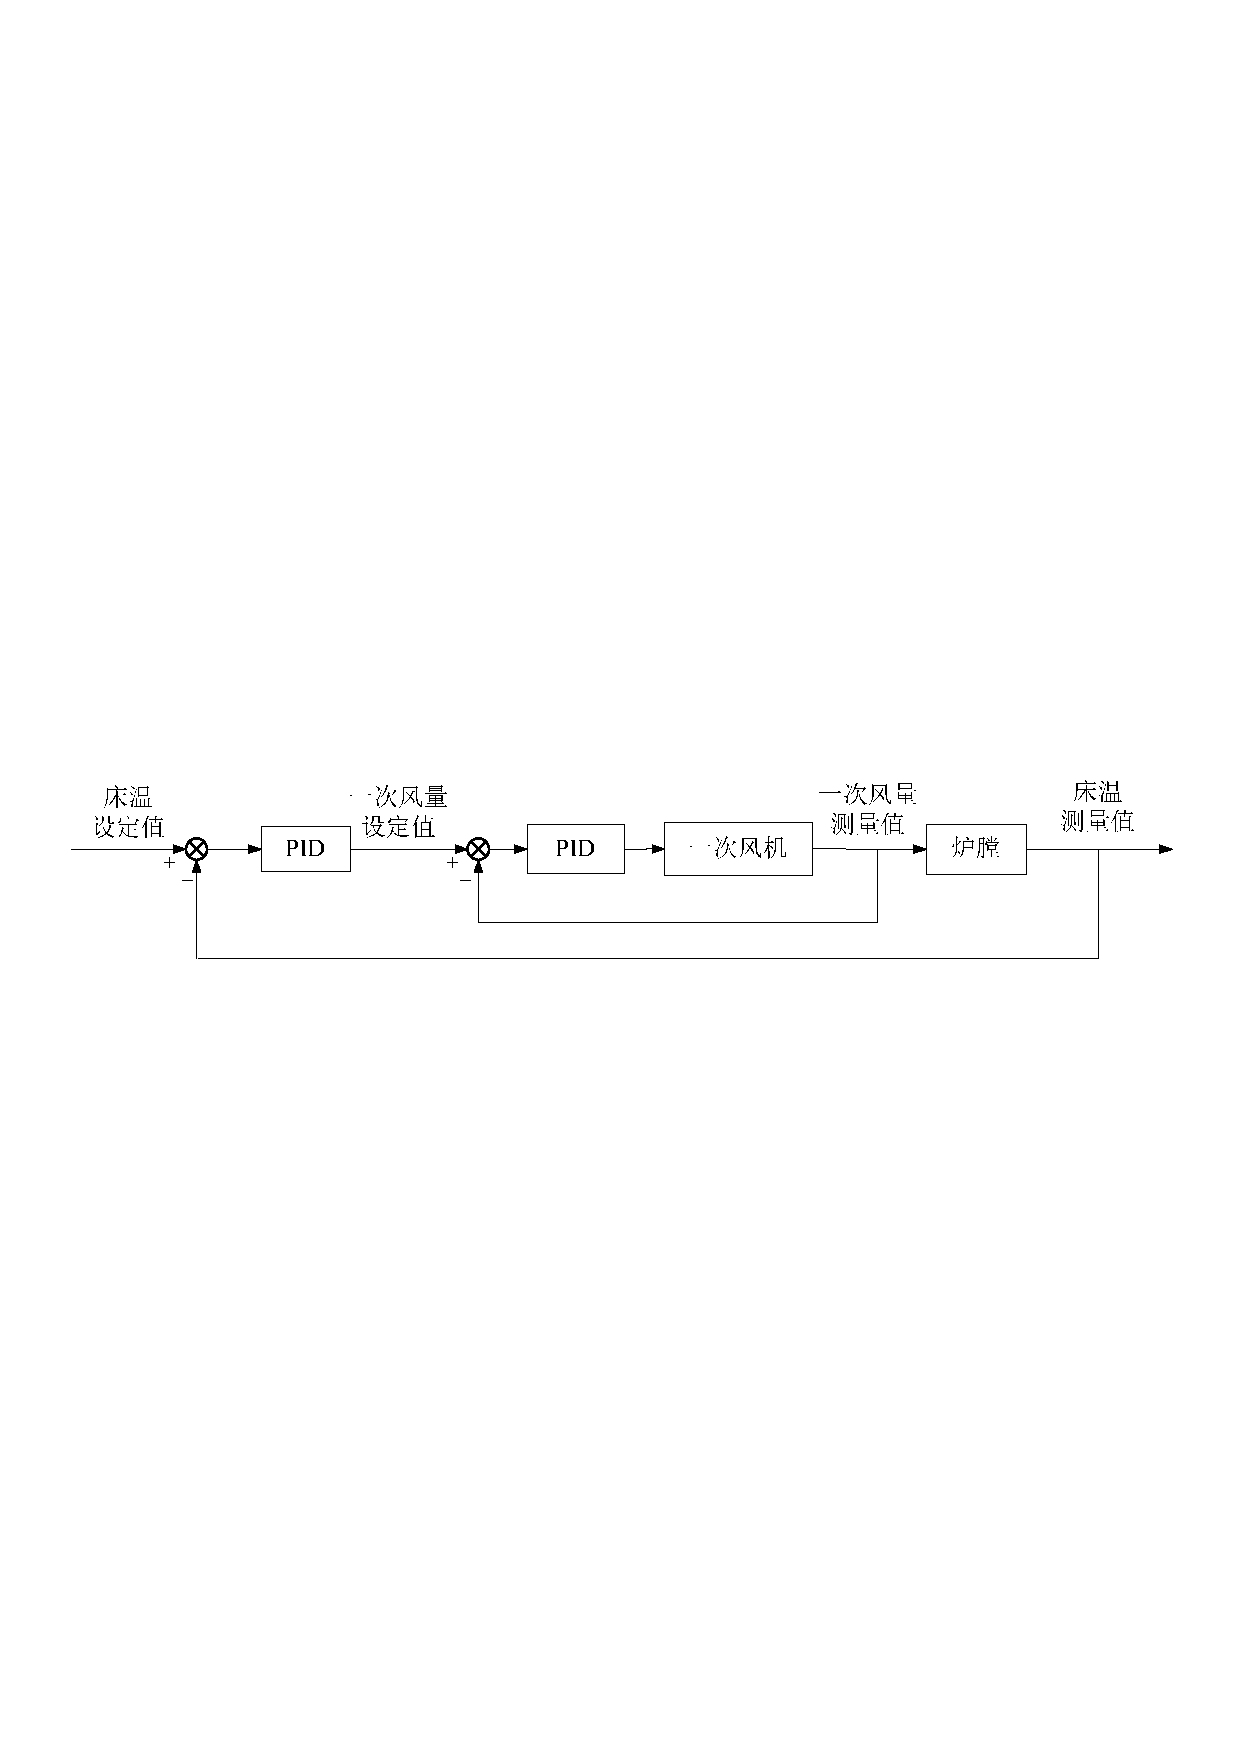
\includegraphics[width=13cm]{bed_tem_pid}
\caption{床温回路PID控制策略} \label{fig:bed_tem_pid}
\end{figure}

\begin{figure}[!htb]
\centering
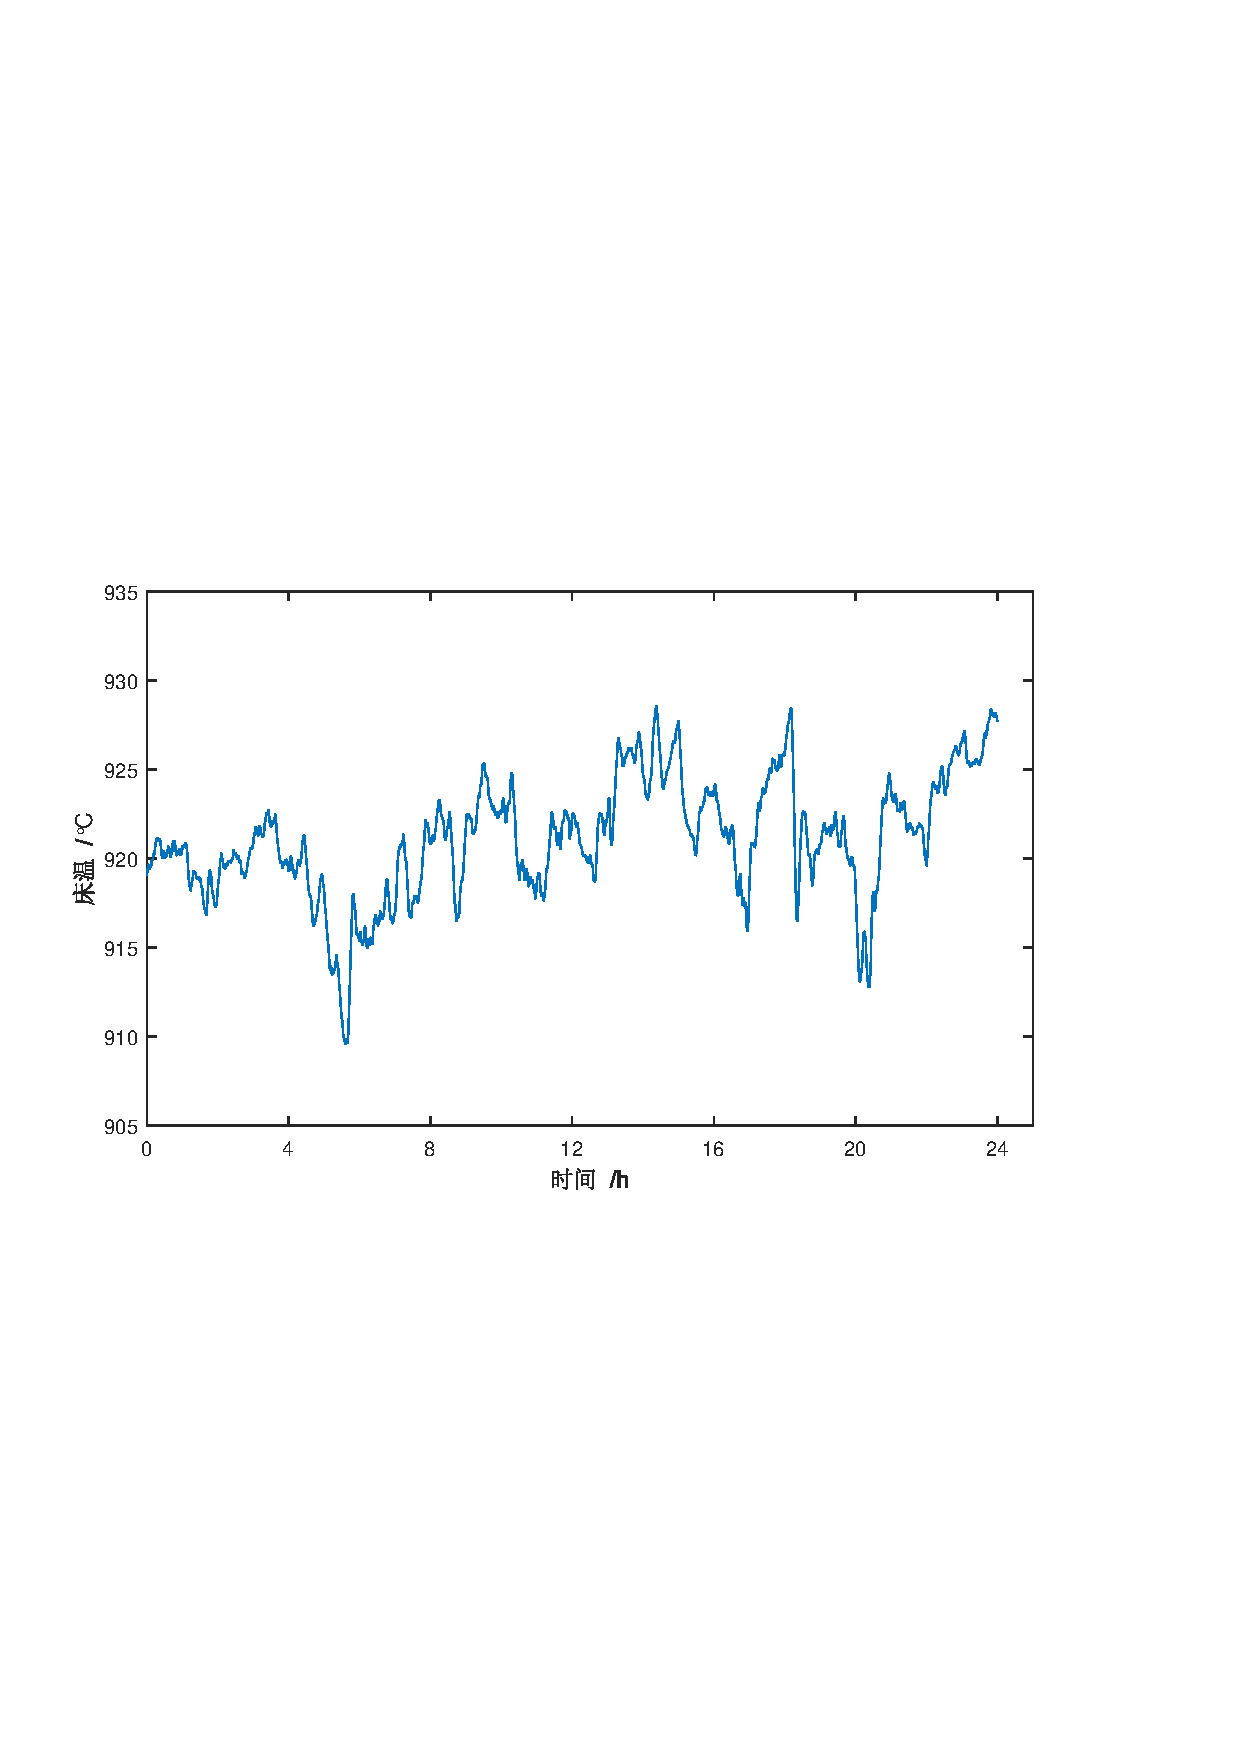
\includegraphics[width=12cm]{bed_tem_line_pid}
\caption{床温回路控制效果} \label{fig:bed_tem_line_pid}
\end{figure}
 
某日床温曲线如图~\ref{fig:bed_tem_line_pid}~所示。床温基本维持在910$\,$\si{\degreeCelsius}~到930$\,$\si{\degreeCelsius}~之间。但是床温一直处于较大波动状态。在约4时床温开始下降,直到910$\,$\si{\degreeCelsius},,随后又开始快速上升到920$\,$\si{\degreeCelsius},之后床温开始出现较大程度的振荡。在18时床温达到了930$\,$\si{\degreeCelsius},接近高限935$\,$\si{\degreeCelsius},随后又在20时下降到910$\,$\si{\degreeCelsius}。



\subsection{床层压差回路}

床层压差反映了循环流化床锅炉炉膛内密相区的床料厚度。循环流化床锅炉的正常运行要求维持一定的床层厚度。料层过薄的话容易被流化风吹穿,进而导致床料燃烧分布不均匀引起局部结渣。由于灰渣没有完全燃烧,含碳量较高,锅炉的热效率也会降低。料层过厚会引起水冷风室压力过高,密相区底部大颗粒物料堆积,堵塞流化风压头,危及锅炉的安全运行。由于炉膛内处于流化状态,没有明显的料位高度,床层厚度只能通过床层压差及一次风量估算。锅炉正常运行情况下,床层厚度应保持500$\,$\si{\mm}~左右,床层压差应保持在5$\,$\si{\kilo\pascal}~到10$\,$\si{\kilo\pascal}。
 
目前床层压差的控制是通过调节冷渣机转速来实现的,采用单回路调节,控制器为PID控制器,如图~\ref{fig:bed_pre_pid}。没有考虑给煤量和石灰石量的波动对床层压差的影响。在锅炉负荷波动不大的情况下,给煤量波动不大,这个回路是没有什么问题的。但当给煤量和石灰石量波动较大时,单纯依靠冷渣机转速来控制床层压差,床层压差会出现较大波动。

\begin{figure}[!htb]
\centering
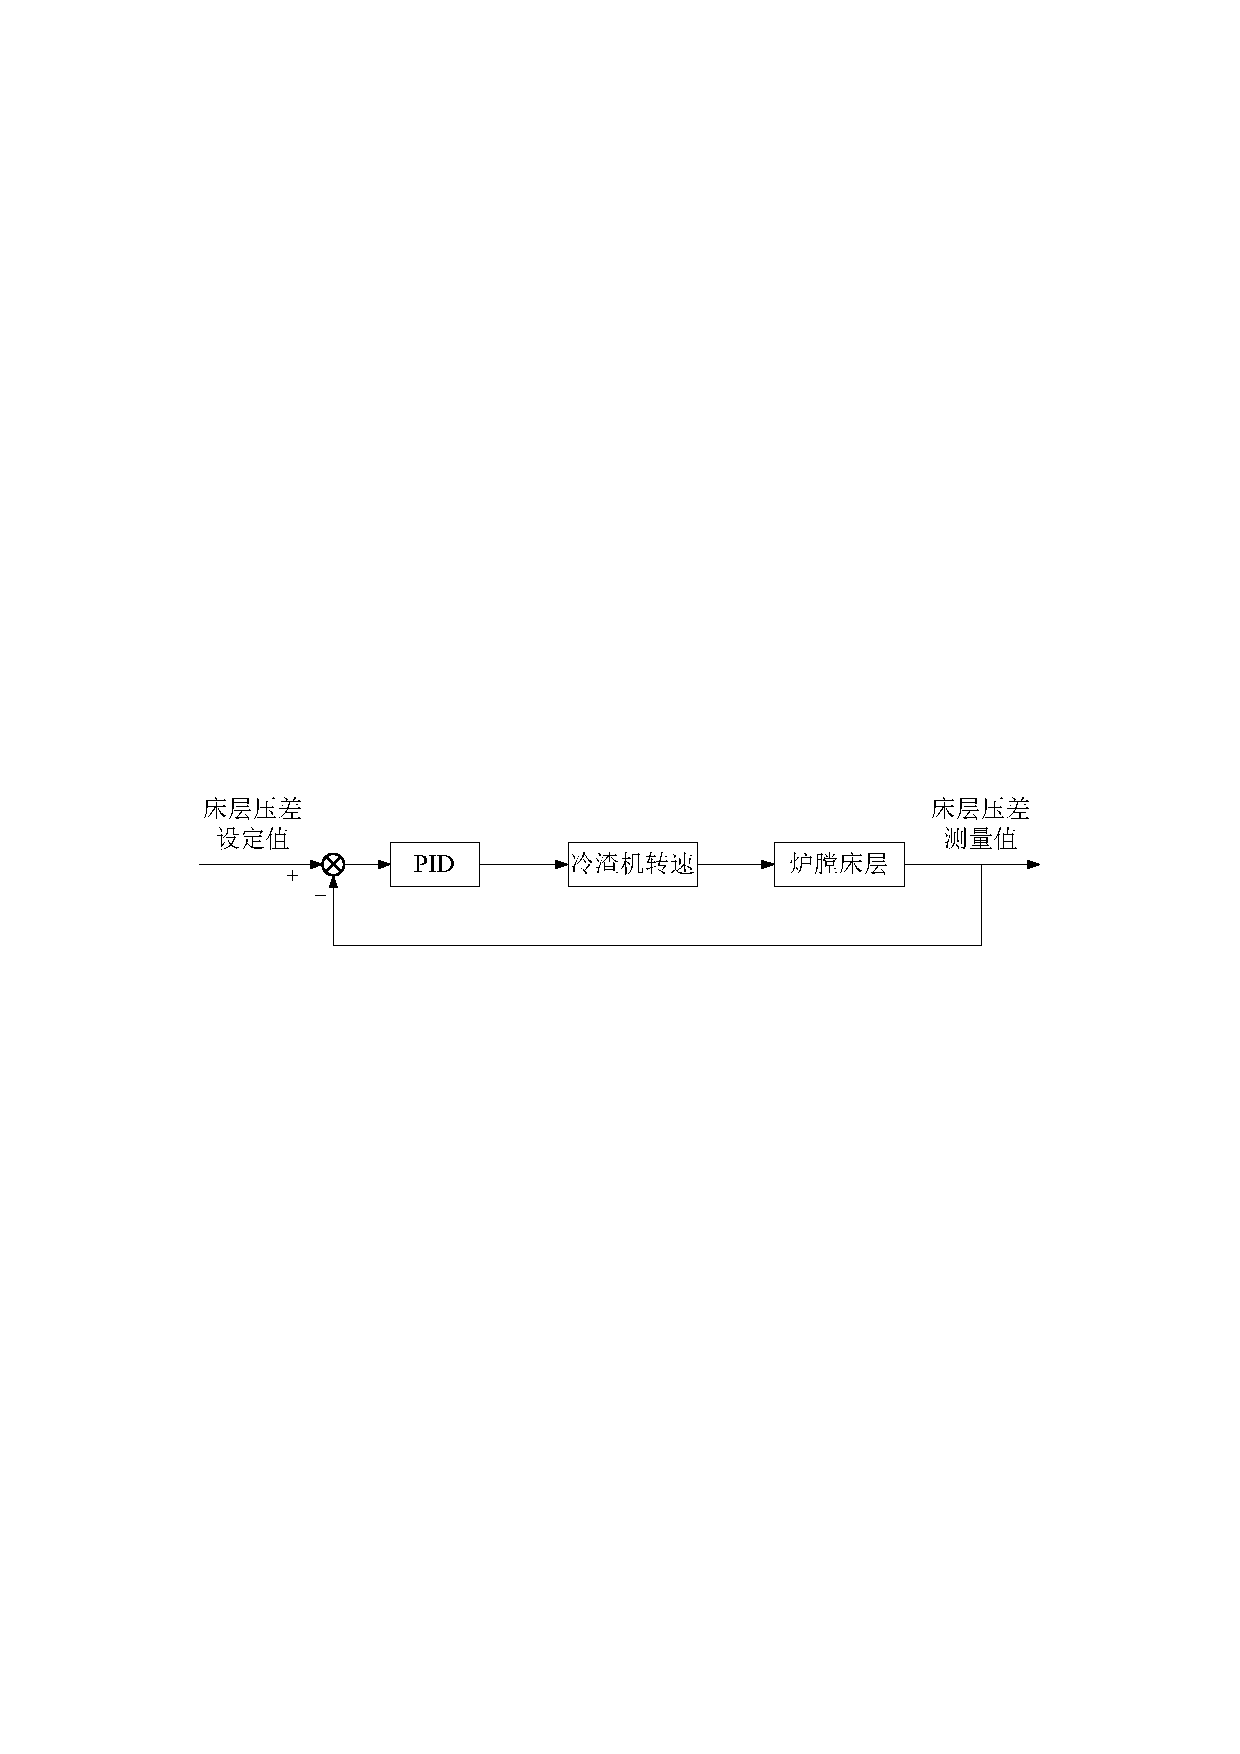
\includegraphics[width=13cm]{bed_pre_pid}
\caption{床层压差回路PID控制策略} \label{fig:bed_pre_pid}
\end{figure}


\begin{figure}[hbtp]
\centering
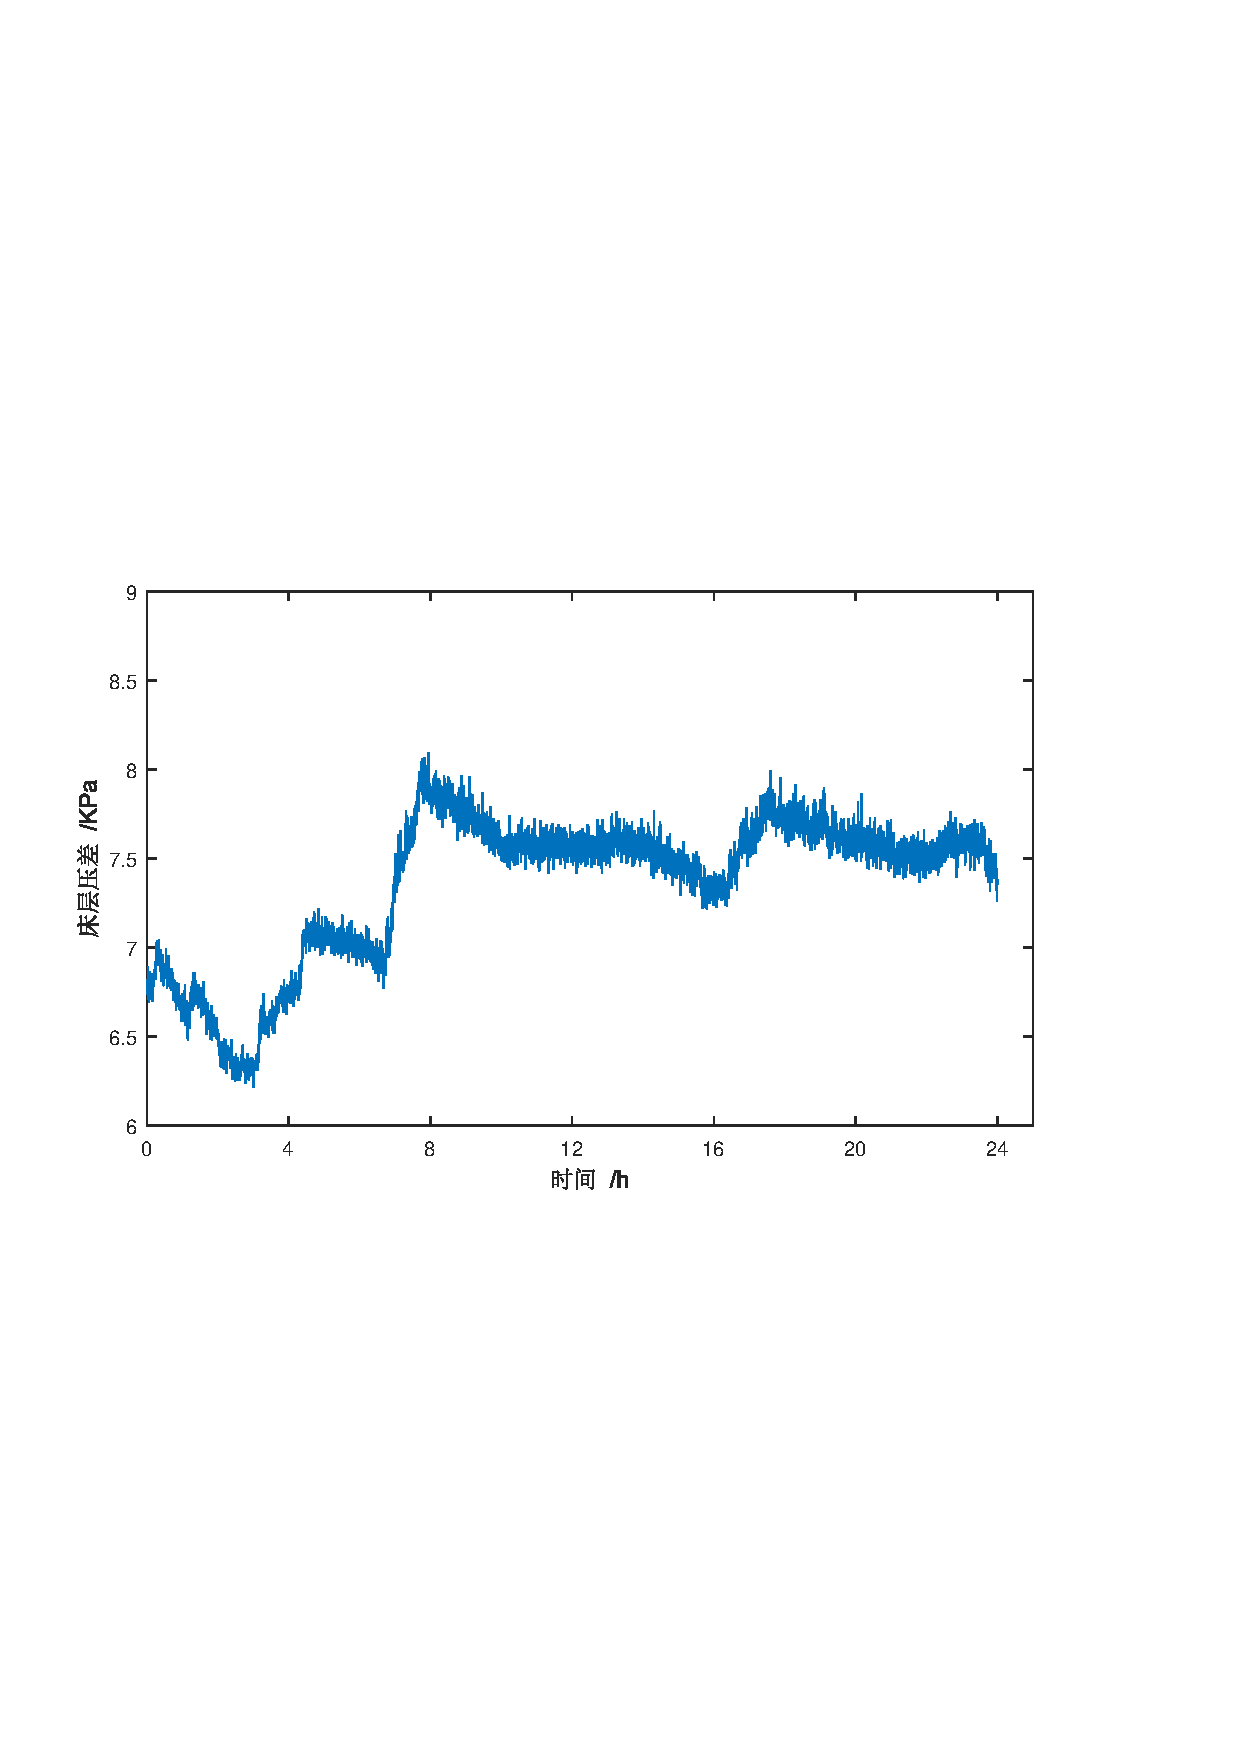
\includegraphics[width=12cm]{bed_pre_line_pid}
\caption{床层压差回路控制效果} \label{fig:bed_pre_line_pid}
\end{figure}
 
某日床层压差曲线如图~\ref{fig:bed_pre_line_pid}~所示。可以看出全天床层压差的波动幅度2$\,$\si{\kilo\pascal}~左右。从开始床压下降到6.2$\,$\si{\kilo\pascal}~,调节到7.2$\,$\si{\kilo\pascal}~后又出现压差的下滑的趋势,随后调节到8.2$\,$\si{\kilo\pascal}~后压差再次下滑,基本上不断向上调节,又不断下滑。虽然生产工艺允许压差的较大幅度波动,但失控的压差容易导致床层流化状态的不稳定,增加燃烧系统的控制难度。


\section{氮氧化物测量现状}
\label{sec:nox_measure_now}
\ce{NOx}是燃煤电站排放的主要污染物之一。在脱硝系统中,系统通过调节氨水和稀释水的流量来控制~\ce{NOx}浓度,氨水和稀释水的流量是由烟道~\ce{NOx}测定值与~\ce{NOx}设定值的偏差计算的。因此,烟道~\ce{NOx}排放量的测量对脱硝系统的控制有着重要影响。除此之外,~\ce{NOx}测量的准确性也会影响燃煤电厂脱硝电价补贴的核算。


\ce{NOx}由~\ce{NO}和~\ce{NO2}组成,因此其测量也依托于~\ce{NO}和~\ce{NO2}的测量技术。~\ce{NO}的测量主要依靠化学发光法,~\ce{NO2}的测量主要依靠湿化学法和光谱法。这些方法测定灵敏度高、检出限低,但测量过程需要将~\ce{NOx}完全转化为~\ce{NO}或~\ce{NO2},装置复杂,价格昂贵,且测量耗时较长。相对而言,~\ce{NOx}化学传感器能满足工业现场连续监测的要求。根据测量原理的不同,~\ce{NOx}化学传感器又分为声表面波~\ce{NOx}传感器、~\ce{NOx}光纤传感器、半导体~\ce{NOx}传感器和~\ce{NOx}电化学传感器\cite{王康丽2003氮氧化物化学传感器}。

\begin{figure}[hbtp]
\centering
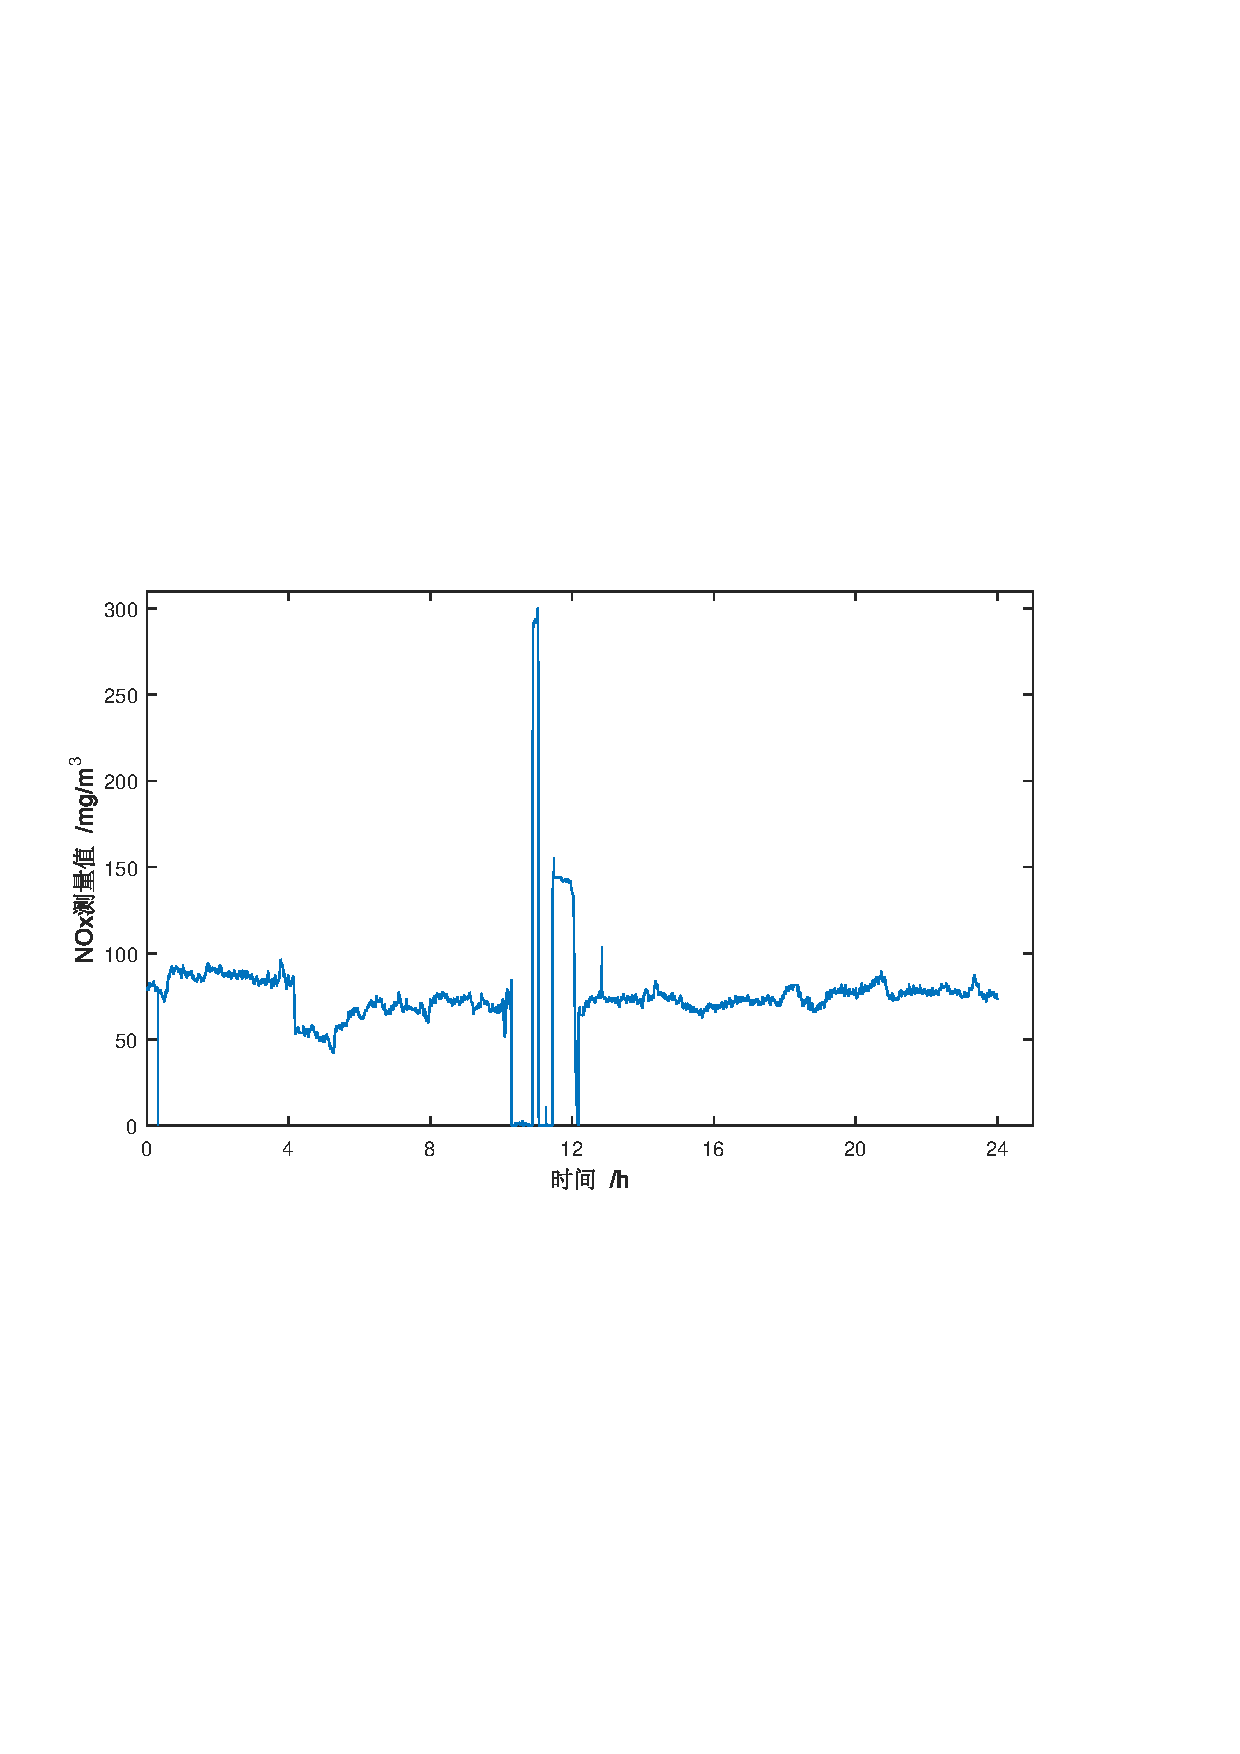
\includegraphics[width=12cm]{nox_measure}
\caption{现场~\ce{NOx}测量现状} \label{fig:nox_measure}
\end{figure}

独山子热电厂采用氧化锆探头作为~\ce{NOx}测量装置,该传感器属于固态电解质电化学传感器,选择专一性好且结构紧凑,适用于工业现场连续监测。但由于氧化锆材料的稳定性和工业现场复杂工作环境,存在性能劣化、机械性差、电势异常、电极脱落、寿命短等问题\cite{罗顺安2010氧化锆}。分析DCS系统记录的历史数据可以发现,~\ce{NOx}传感器的故障往往导致脱硝回路的异常运行。如图~\ref{fig:nox_measure}~所示,~\ce{NOx}传感器出现了三次故障,故障时段~\ce{NOx}测量值记录为0,故障时间长达1$\,$\si{\hour}。由于传感器发生故障,脱硝装置运行异常,导致当日部分时段~\ce{NOx}排放量达到了300$\,$\si[per-mode=symbol]{\mg\per\m^3},是国家规定限定值的3倍。


 
因此,有必要改进现场~\ce{NOx}测量方法,尽可能避免传感器故障对脱硝系统的影响。

\section{本章小结}
本章首先简要介绍了现场锅炉的设计参数、主要结构、运行工艺及现场采用的DCS系统。随后分析了当前燃烧系统的控制策略和控制水平,可以看出控制策略存在一定的问题,原有的自动控制系统基本失效,燃烧系统处于手动控制状态。最后结合现场实际测量数据分析了~\ce{NOx}传感器存在的问题,指出提高其测量水平的必要性。